\documentclass[a4paper,12pt]{article}
\usepackage{graphicx}
\usepackage[UTF8]{ctex}
\usepackage{fontspec}
\usepackage{booktabs}
\usepackage{float}%浮动体
\usepackage{amsmath,amssymb}
\usepackage{fancyhdr}
%\usepackage{xcolor}
\usepackage{colortbl}
\usepackage{geometry}
\geometry{top=2cm,bottom=2cm,left=1cm,right=1cm}
\begin{document}
	\begin{figure}[H]
	\begin{center}
		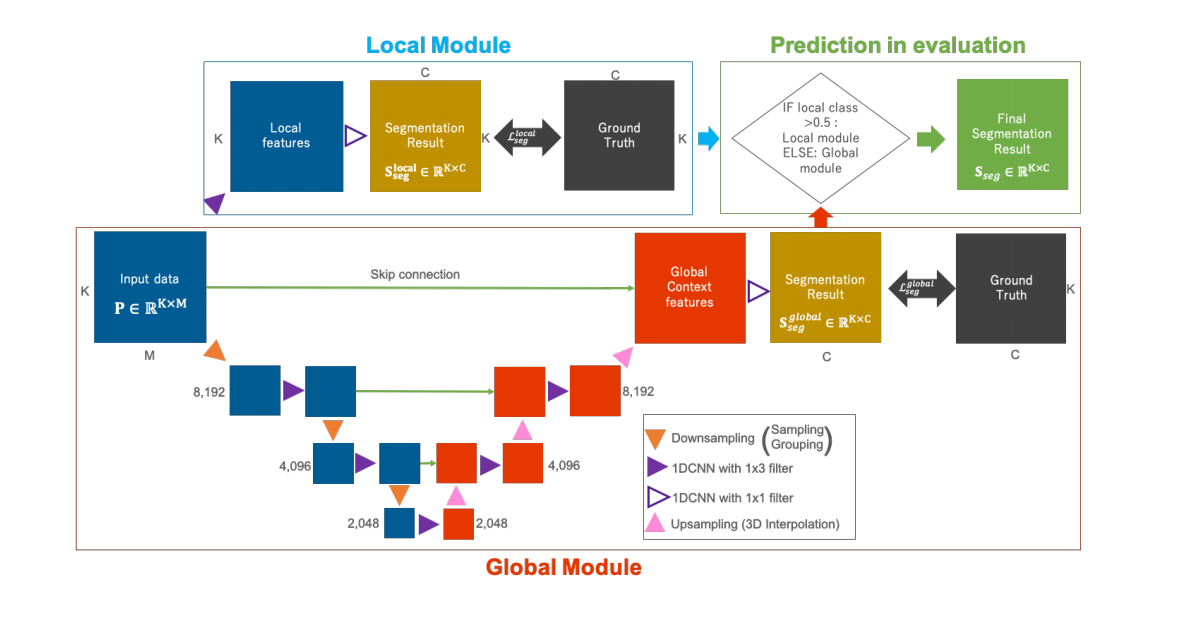
\includegraphics[width=0.9\textwidth]{img/LiDaSeg_Hiera.png} 
		\caption{LiDaSeg\_Hiera}
	\end{center}
\end{figure}

\textbf{分析}:
\begin{itemize}
	\item Local Module (input: waveform --> segmentation results)
	\item Global Module(input: x,y,z and waveform --> segmentation results)
\end{itemize}
由于类别的分布不均匀,大部分是分类是背景,造成分类的错误,给不同的类别赋予权重,某类的比例大的权重就小
$$\lambda_{c}=\frac{1}{\ln \left(\alpha+\frac{K_{c}}{\sum_{c=1}^{C} K_{i}}\right)}$$
$$\mathcal{L}_{s e g}=\sum_{i=1}^{K} \sum_{c=1}^{C} \lambda_{c} t_{i, c} \log s_{i, c}$$
总的$$loss = \mathcal{L}_{s e g}^{local} + \mathcal{L}_{s e g}^{global}$$

\paragraph{语义分割} 如图1

\end{document}